% !TeX program = xelatex
% 第二研究ノート: equal disk circle packing, exact lemmas and open global certificate
\documentclass[11pt,a4paper]{article}
\usepackage[margin=22mm,top=22mm,bottom=23mm]{geometry}
\usepackage{fontspec,xeCJK}
\setmainfont{Liberation Serif}
\setsansfont{Liberation Sans}
\setmonofont{DejaVu Sans Mono}[Scale=.85]
\setCJKmainfont{Noto Serif CJK JP}
\setCJKsansfont{Noto Sans CJK JP}
\setCJKmonofont{Noto Sans Mono CJK JP}
\usepackage{amsmath,amssymb,amsthm,mathtools}
\usepackage{microtype,booktabs,array,tabularx,multirow,longtable}
\usepackage{tikz}
\usetikzlibrary{arrows.meta,calc,angles,quotes,decorations.pathreplacing,patterns,positioning,backgrounds,fit,shapes.geometric}
\usepackage[most]{tcolorbox}
\usepackage{enumitem,caption,fancyhdr,hyperref,cleveref,needspace,float}
\usepackage{xcolor}
\hypersetup{colorlinks=true,linkcolor=blue!55!black,urlcolor=blue!60!black,citecolor=blue!55!black,pdftitle={15等円最小外接円パッキング：第二研究ノート},pdfauthor={Working research note}}
\definecolor{ink}{HTML}{183552}
\definecolor{sea}{HTML}{317D9E}
\definecolor{amber}{HTML}{BE7E3E}
\definecolor{mint}{HTML}{38715F}
\definecolor{faint}{HTML}{F1F5F8}
\definecolor{alert}{HTML}{9F3E45}
\renewcommand{\arraystretch}{1.18}
\setlength{\parindent}{1em}
\setlength{\parskip}{3pt}
\setlist[itemize]{itemsep=2pt,topsep=4pt,leftmargin=2em}
\newtheoremstyle{JPthm}{6pt}{6pt}{\normalfont}{}{\bfseries\color{ink}}{.}{.65em}{}
\theoremstyle{JPthm}
\newtheorem{theorem}{定理}[section]
\newtheorem{lemma}[theorem]{補題}
\newtheorem{proposition}[theorem]{命題}
\newtheorem{corollary}[theorem]{系}
\theoremstyle{definition}
\newtheorem{definition}[theorem]{定義}
\newtheorem{problem}[theorem]{未解決課題}
\renewcommand{\proofname}{証明}
\newcommand{\Rstar}{R_{15}^{*}}
\newcommand{\Rc}{R_{0}}
\newcommand{\thzero}{\theta_{0}}
\newcommand{\azero}{a_{0}}
\newcommand{\bzero}{b_{0}}
\newtcolorbox{statusbox}[1][]{colback=faint,colframe=sea!55!black,boxrule=.65pt,arc=2pt,top=7pt,bottom=7pt,left=9pt,right=9pt,#1}
\newtcolorbox{warningbox}[1][]{colback=red!2,colframe=alert!63,boxrule=.7pt,arc=2pt,top=8pt,bottom=8pt,left=9pt,right=9pt,#1}
\newtcolorbox{keybox}[1][]{colback=white,colframe=ink!70,boxrule=.85pt,arc=2pt,top=8pt,bottom=8pt,left=9pt,right=9pt,#1}
\captionsetup{font=small,labelfont={bf,color=ink},skip=5pt}
\pagestyle{fancy}\fancyhf{}
\fancyhead[L]{\sffamily\footnotesize 15等円の最小外接円：第二研究ノート}
\fancyhead[R]{\sffamily\footnotesize 2026-10-09}
\fancyfoot[C]{\thepage}
\setlength{\headheight}{15pt}
\tikzset{innerdisk/.style={draw=ink!75,fill=amber!42,line width=.65pt},outerdisk/.style={draw=ink!75,fill=sea!27,line width=.65pt},guideline/.style={draw=ink!45,densely dashed,line width=.65pt},flowbox/.style={draw=ink!80,rounded corners=2pt,fill=faint,inner sep=6pt,font=\small\sffamily,align=center},figlabel/.style={font=\footnotesize\sffamily,fill=white,inner sep=1pt}}
\begin{document}
\begin{center}
{\sffamily\color{ink}\LARGE\bfseries 15等円の最小外接円パッキング}\par
\vspace{2mm}{\sffamily\large 第二研究ノート：壁面化・半径順位・角度予算と大域排除}\par
\vspace{3mm}{\color{sea}\rule{.75\linewidth}{1pt}}\par\vspace{2mm}
{\small 2026年10月9日\quad ／\quad 第1ノートの続編・独立に読める版}
\end{center}
\begin{warningbox}
\textbf{研究状況：15等円の大域最適性は依然として未証明である。}\par
本稿の定理は、特定の半径範囲または内外配置に関する\emph{必要条件・部分的排除}である。
760種の内外巡回パターンに属するすべての連続的な半径配置を排除する
厳密な証明書は、現時点では構成していない。
\end{warningbox}
\begin{abstract}
半径1の合同円15個を最小の円形容器に収納する問題を考える。
最良既知の候補半径は
$\Rc=1+\sqrt{1+(2+\cot(\pi/5))^2}\approx4.5213569647$ である。
第1ノートで得た半径しきい値 $L$ と内外分類を発展させ、
外側に分類されたすべての円を偏角を保ったまま半径 $\bzero=\Rc-1$ の円周へ移せることを厳密に示す。
したがって、容器半径 $R\le\Rc$ の非実現可能性判定は内側5--8円の中心距離だけに帰着できる。
また、順位統計量に対する幾何学的上下界を導き、
内側5円・外側10円の場合には壁面角度予算から
「内側5円が一斉に $\azero=\csc(\pi/5)$ 以上」または「一斉に以下」
という二つの大域領域を排除する。
残る混合領域および内側6--8円の場合の完全排除は未解決である。
\end{abstract}
\tableofcontents
\clearpage
\section{定式化と候補配置}
中心 $p_i\in\mathbb R^2$ を持つ15個の単位円が半径 $R$ の容器に収まる条件は
\begin{equation}\label{eq:feasibility}
 \|p_i\|\le R-1,\qquad \|p_i-p_j\|\ge2\quad(i\ne j).
\end{equation}
最適容器半径を $\Rstar$ とする。
\begin{definition}[基準定数]\label{def:constants}
\begin{align}
 \phi&=\frac\pi5, &\azero&=\frac1{\sin\phi},\\
 \bzero&=\sqrt{1+(2+\cot\phi)^2}, &\Rc&=1+\bzero,\\
 L&=\bzero-\frac4{\bzero},&\thzero&=2\arcsin\frac1{\bzero},\\
 \alpha_0&=\phi-\arcsin\frac1{\bzero}, & \gamma_0&=2\arcsin\frac1L.
\end{align}
数値的には、
$\azero\approx1.701301617$, $\bzero\approx3.521356965$,
$L\approx2.385431229$, $\thzero\approx32.995947^\circ$,
$\alpha_0\approx19.502026^\circ$ である。
\end{definition}
候補配置の中心は、極座標で
\begin{equation}\label{eq:candidate}
 I_k=(\azero,2k\phi),\quad
 O_k^{\pm}=(\bzero,2k\phi\pm\alpha_0),\qquad k=0,\ldots,4.
\end{equation}
この配置のすべての非重複条件は余弦定理で直接検証でき、
\begin{equation}\Rstar\le\Rc\end{equation}
が厳密に従う。これは既知の最良配置に対応する\emph{上界}である\cite{packomania}。
同じ円形容器問題については14等円の最適性を証明する研究もある\cite{ekanayake}。
\begin{figure}[H]\centering
\begin{tikzpicture}[scale=.68]
\pgfmathsetmacro{\a}{1/sin(36)}\pgfmathsetmacro{\b}{sqrt(1+(2+1/tan(36))^2)}
\pgfmathsetmacro{\al}{36-asin(1/\b)}
\draw[ink,thick,fill=sea!3] (0,0) circle[radius={1+\b}];
\draw[guideline] (0,0) circle[radius=\b];
\draw[guideline] (0,0) circle[radius=\a];
\foreach \k in {0,...,4}{
\pgfmathsetmacro{\t}{90+72*\k}
\draw[innerdisk] (\t:\a) circle[radius=1];
\draw[outerdisk] ({\t-\al}:\b) circle[radius=1];
\draw[outerdisk] ({\t+\al}:\b) circle[radius=1];}
\node[figlabel,anchor=west] at (4.45,2.9) {$I$: 内側5円};
\draw[amber,thick,-{Latex}] (4.37,2.70)--(1.0,1.8);
\node[figlabel,anchor=west] at (4.45,2.0) {$O$: 外側10円};
\draw[sea,thick,-{Latex}] (4.37,1.8)--(3.35,.9);
\node[figlabel,anchor=west] at (4.45,0.0) {$R_0=1+b_0$};
\end{tikzpicture}
\caption{15等円の既知 $D_5$ 対称配置。\emph{この対称性を任意の配置に仮定してはならない}。}
\end{figure}

\section{外側円を一括で壁面に押し出す補題}
\subsection{余弦四隅評価}
中心半径 $x,y>0$ の単位円ペアに対し
\begin{equation}\label{eq:cxy}
 c(x,y)=\frac{x^2+y^2-4}{2xy}
\end{equation}
とおく。中心角 $\Delta$ の非重複条件は $\cos\Delta\le c(x,y)$ である。
\begin{lemma}[半径箱における余弦の四隅評価]\label{lem:corner}
正数 $0<\ell\le u$ に対し、$c(x,y)$ の $[\ell,u]^2$ 上の最大値は四隅のいずれかにある。
\end{lemma}
\begin{proof}
$y$ を固定すると
\[
 \frac{\partial c}{\partial x}=\frac{x^2-y^2+4}{2x^2y}.
\]
分子は $x$ について単調増加するから、$c$ は内部に局所最大を持たない
（極値があるとすれば最小）。したがって $x$ に関する最大値は端点で達成される。
同じ議論を $y$ に適用すれば、最大値は四隅に帰着する。
\end{proof}
\begin{lemma}[外側箱の最大余弦]\label{lem:wallcos}
基準定数 $L,\bzero$ について
\begin{equation}\label{eq:boxbound}
\max_{L\le x,y\le\bzero}c(x,y)=c(\bzero,\bzero)=1-\frac2{\bzero^2}.
\end{equation}
\end{lemma}
\begin{proof}
\Cref{lem:corner}を用いる。対角端点では
$c(L,L)=1-2/L^2<c(\bzero,\bzero)$。
また $L=\bzero-4/\bzero$ を代入すると
\[
 c(L,\bzero)=c(\bzero,L)=c(\bzero,\bzero).
\]
これで四隅の大小が確定する。
\end{proof}
\begin{theorem}[外側円の壁面化]\label{thm:radialpush}
$R\le\Rc$ の配置において、中心半径 $s_i=\|p_i\|$ が $s_i\ge L$ を満たす
すべての円を、偏角を変えず、中心半径 $\bzero$ まで移しても非重複は保たれる。
したがって、容器半径 $\Rc$ 内では外側円をすべて壁面接触にしてよい。
\end{theorem}
\begin{proof}
外側同士のペア $(i,j)$ について、元の非重複条件と\Cref{lem:wallcos}より
\[
\cos\Delta_{ij}\le c(s_i,s_j)\le c(\bzero,\bzero).
\]
右端は、両円を中心半径 $\bzero$ に移した後の非重複条件そのものである。
内側中心半径 $x<L$ と外側中心半径 $y\ge L$ のペアについて、中心角を $\Delta$ とすると
\[
D^2(x,y,\Delta)=x^2+y^2-2xy\cos\Delta,
\quad
\frac{\partial D^2}{\partial y}=2(y-x\cos\Delta)>0
\]
である。よって外側を押し出すと内外間の距離は増加する。
すべての外側ペアと内外ペアを同時に確認したので主張が従う。
\end{proof}
\begin{figure}[H]\centering
\begin{tikzpicture}[scale=.92]
\draw[ink,thick] (0,0) circle[radius=2.39];
\draw[guideline] (0,0) circle[radius=1.5];
\draw[guideline] (0,0) circle[radius=2.0];
\draw[ink] (0,0) -- (27:2.2);
\draw[innerdisk] (128:1.04) circle[radius=.36];
\draw[outerdisk] (27:1.62) circle[radius=.36];
\draw[outerdisk] (27:2.0) circle[radius=.36];
\draw[amber,very thick,-{Latex[length=3mm]}] (27:1.69)--(27:1.96);
\draw[guideline] (27:1.62)--(128:1.04);
\draw[sea,thick] (27:2.0)--(128:1.04);
\node[figlabel] at (3.25,1.30) {外側円 $y\mapsto b_0$};
\node[figlabel] at (3.15,.62) {偏角を固定};
\node[figlabel] at (-2.9,-1.7) {内外間距離は減少しない};
\end{tikzpicture}
\caption{内側・外側ペアの押し出し。外側同士については円周角度の四隅評価が必要。模式図であり実寸ではない。}
\end{figure}
\begin{statusbox}
\textbf{次元削減：} 内側の円が $k$ 個なら、円周へ押し出した後に残る\emph{自由な中心半径}は $k$ 個のみ。
角度差変数は負閉路検査により除去できる。\par
第1ノートの分類 $k\in\{5,6,7,8\}$ と組み合わせると、
15変数の半径問題から\emph{最大8変数}へ縮小する。
\end{statusbox}

\section{内外の個数と中心半径の順位統計量}
\begin{lemma}[内側5--8円への分類]\label{lem:class}
$R\le\Rc$ の任意の実現可能配置について、
\[
5\le\#\{i:\|p_i\|<L\}\le8.
\]
\end{lemma}
\begin{proof}
外側ペアの角度分離は\Cref{lem:wallcos}から少なくとも
$\thzero=2\arcsin(1/\bzero)$。したがって
$11\thzero>2\pi$ より、外側は最大10円である。
内側に9円あれば、9円は半径 $L+1\approx3.385431$ の容器に入る。
一方、既知の9等円の最適半径は約 $3.613126$ であり、これに反する\cite{packomania}。
よって内側は5--8円である。
\end{proof}
中心距離を昇順に
\[
 0\le s_{(1)}\le\cdots\le s_{(15)}\le\bzero
\]
と並べる。$R_k^*$ を $k$ 等円の最適容器半径とすれば、任意の $k$ について
\begin{equation}\label{eq:orderlower}
 s_{(k)}\ge R_k^*-1.
\end{equation}
これは最も内側の $k$ 円のみを取り出せば直ちに従う。

\begin{proposition}[外側集団からの順位上界]\label{prop:orderupper}
$m\in\{11,12,13,14,15\}$ に対して
\begin{equation}\label{eq:um}
 u_m=\bzero\cos\frac{2\pi}{m}
 -\sqrt{4-\bzero^2\sin^2\frac{2\pi}{m}}
\end{equation}
とおく。このとき
\[
 \boxed{s_{(16-m)}\le u_m}.
\]
\end{proposition}
\begin{proof}
上位 $m$ 個の中心半径がすべて $u>u_m$ だと仮定する。
その中心半径は $[u,\bzero]$ にある。\Cref{lem:corner} と
$c(u_m,\bzero)=\cos(2\pi/m)$ から、
$m=11,\ldots,15$ の各場合に
\[
 \max_{u\le x,y\le\bzero}c(x,y)<\cos\frac{2\pi}{m}
\]
が従う（$c(\bzero,\bzero)<\cos(2\pi/m)$、
$c(u_m,u_m)<\cos(2\pi/m)$ を代入して確認する）。
よってどのペアも中心角が $2\pi/m$ より大きく、
$m$ 個の角度ギャップの総和が $2\pi$ を超える。矛盾。
\end{proof}
\begin{table}[H]\centering\small
\caption{中心距離の厳密公式\eqref{eq:um}から得られる上界。小数は表示用。}
\begin{tabular}{@{}cccc@{}}\toprule
上位 $m$ 円 & 制約される順位 & 上界 $u_m$ & 近似値\\\midrule
15 & $s_{(1)}$ & $u_{15}$ & 1.820991\\
14 & $s_{(2)}$ & $u_{14}$ & 1.882034\\
13 & $s_{(3)}$ & $u_{13}$ & 1.968219\\
12 & $s_{(4)}$ & $u_{12}$ & 2.100895\\
11 & $s_{(5)}$ & $u_{11}$ & 2.349503\\\bottomrule
\end{tabular}
\end{table}
\begin{figure}[H]\centering
\begin{tikzpicture}[x=.92cm,y=.92cm]
\draw[ink,-{Latex}] (0,0)--(8,0) node[right,figlabel] {中心半径};
\foreach \x/\lab in {0/{0},2.0/{a_0},4.8/{L},7.25/{b_0}} {
  \draw[ink!55] (\x,-.14)--(\x,.15);\node[font=\scriptsize] at (\x,-.37) {$\lab$};}
\fill[amber!18] (0,.55) rectangle (4.8,1.45);
\fill[sea!17] (4.8,.55) rectangle (7.25,1.45);
\node at (2.4,1.0) {内側（5--8個）};
\node at (6.03,1.0) {外側（7--10個）};
\draw[sea,very thick,-{Latex[length=2mm]}] (5.05,1.85)--(7.18,1.85);
\node[font=\small] at (6.15,2.10) {すべて $b_0$ へ壁面化};
\draw[amber,very thick] (3.08,2.48)--(4.4,2.48);
\node[font=\small,anchor=west] at (4.5,2.48) {$s_{(5)}\le u_{11}<L$};
\end{tikzpicture}
\caption{順位上界と内外分類の模式図。$s_{(5)}\le u_{11}<L$ は、少なくとも5円が内側にあることを別経路から保証する。}
\end{figure}
さらに $s_{(1)}+s_{(2)}\ge2$ より、
\begin{equation}\label{eq:firstpositive}
 s_{(1)}\ge2-u_{14}>0.
\end{equation}
従って、この半径範囲の15円配置では\emph{原点に中心を持つ円は存在しない}。

\section{外側10円の角度予算}
\Cref{thm:radialpush}によって、10個の外側円をすべて中心半径 $\bzero$ に置ける。
外側の隣接2円は、少なくとも $\thzero$ の中心角を必要とする。
10個の外側ギャップ $g_j$ は
\begin{equation}\label{eq:sumgaps}
 g_j\ge\thzero,\quad \sum_{j=1}^{10}g_j=2\pi,
 \quad g_j\le2\pi-9\thzero.
\end{equation}
\[
\thzero\approx32.995947^\circ,\qquad
2\pi-9\thzero\approx63.036475^\circ.
\]
\begin{figure}[H]\centering
\begin{tikzpicture}[scale=1.05]
\draw[ink,thick] (0,0) circle[radius=1.88];
\foreach \k in {0,...,9}{\pgfmathsetmacro{\t}{90+36*\k}\fill[sea] (\t:1.88) circle[radius=.085];}
\draw[sea,very thick] (0,0)--(90:1.88);
\draw[sea,very thick] (0,0)--(54:1.88);
\draw[sea!80,-{Latex}] (90:.78) arc[start angle=90,end angle=54,radius=.78];
\node[figlabel] at (.86,1.02) {$g_j$};
\node[figlabel,anchor=west] at (2.3,.9) {10個の外側ギャップ};
\node[figlabel,anchor=west] at (2.3,.35) {$g_j\ge\theta_0$};
\node[figlabel,anchor=west] at (2.3,-.25) {$g_j\le 2\pi-9\theta_0$};
\end{tikzpicture}
\caption{外側10円のみで壁面の角度の大半を消費する。図の点は角度概念を示すもので、実際の最良配置のギャップは等間隔ではない。}
\end{figure}
必要角度の総和から、残る角度余裕は
\begin{equation}\label{eq:budget}
 S_{10}=2\pi-10\thzero\approx30.040528^\circ.
\end{equation}
既知配置では内側各円が1つの外側ギャップを広げ、
\begin{equation}\label{eq:angidentity}
 2\alpha_0+\thzero=2\phi=72^\circ,
 \qquad 2\alpha_0-\thzero\approx6.0081055^\circ
\end{equation}
となる。追加角度が5個でちょうど $S_{10}$ を使い切る。
\begin{figure}[H]\centering
\begin{tikzpicture}[x=1cm,y=1cm]
\node[figlabel] at (1.2,2.35) {内側円のないギャップ};
\fill[sea] (0,1.52) circle (.11);\fill[sea] (3.25,1.52) circle (.11);
\draw[sea,line width=1.5pt] (0,1.52)--(3.25,1.52);
\node[figlabel] at (1.62,1.77) {$\theta_0$};
\node[figlabel] at (1.5,.8) {内側円のあるギャップ};
\fill[sea] (0,0) circle (.11);\fill[amber] (1.65,0) circle (.13);\fill[sea] (3.7,0) circle (.11);
\draw[amber,line width=1.5pt] (0,0)--(1.65,0);
\draw[amber,line width=1.5pt] (1.65,0)--(3.7,0);
\node[figlabel] at (.76,.28) {$\alpha_0$};\node[figlabel] at (2.67,.28) {$\alpha_0$};
\node[figlabel,anchor=west] at (4.2,1.52) {$\theta_0\simeq33.0^\circ$};
\node[figlabel,anchor=west] at (4.2,0) {$2\alpha_0\simeq39.0^\circ$};
\end{tikzpicture}
\caption{ギャップ1個への内側円の挿入は、角度予算を $2\alpha_0-\thzero$ だけ増やす。模式図。}
\end{figure}

\section{内側5円・外側10円の大域的な二領域排除}
本節では内側がちょうど5円の場合を扱い、その中心半径を $a_1,\ldots,a_5<L$ とする。
中心半径 $x,y$ にある単位円ペアの必要な（小さい方の）中心角を
\begin{equation}\label{eq:angle}
 \Phi(x,y)=\arccos\frac{x^2+y^2-4}{2xy}
\end{equation}
と書く（以下の適用範囲では $|x-y|<2<x+y$ が成立する）。
\begin{lemma}[内外角の単調性]\label{lem:alphamon}
$a\in[\azero,L]$ に対して
\[
 \Phi(a,\bzero)\ge\Phi(\azero,\bzero)=\alpha_0.
\]
また $a,a'\in[\azero,L]$ に対して
\[
 \Phi(a,a')\ge\Phi(L,L)=\gamma_0.
\]
\end{lemma}
\begin{proof}
$\partial_a c(a,\bzero)=(a^2-\bzero^2+4)/(2a^2\bzero)<0$
（$L^2<\bzero^2-4$）であるため、$\Phi(a,\bzero)$ は増加する。
後半は\Cref{lem:corner}を箱 $[\azero,L]^2$ に適用し、
四隅を比較すると $c(L,L)$ が最大となることから従う。
\end{proof}
\begin{theorem}[すべての内側半径が $\azero$ 以上なら排除]\label{thm:high}
内側5円・外側10円の配置が $R\le\Rc$ で実現可能であり、
\[
 a_i\ge\azero\qquad(i=1,\ldots,5)
\]
ならば、$R=\Rc$ かつ $a_i=\azero$ がすべての $i$ で成り立つ。
特に $R<\Rc$ の実現可能配置は存在しない。
\end{theorem}
\begin{proof}
\Cref{thm:radialpush}で外側10円を中心半径 $\bzero$ に移す。
各外側ギャップは\eqref{eq:sumgaps}を満たし、幅の最大値は
$2\pi-9\thzero\approx63.0365^\circ$ である。
1つの外側ギャップに内側円が2個以上入ると、
外側--内側、内側--内側、内側--外側の角度下界の和が
\[
2\alpha_0+\gamma_0\approx88.5737^\circ
>2\pi-9\thzero
\]
になり矛盾する。ゆえに、各外側ギャップには内側円を高々1個しか入れられない。
内側円は5個あるから、外側10ギャップの5つにちょうど1個ずつ入る。
空ギャップは少なくとも $\thzero$、内側円1個入りのギャップは少なくとも
$2\alpha_0$ を必要とする。したがって
\[
 2\pi\ge 5\thzero+10\alpha_0
 =2\pi
\]
で、すべて等号である。\Cref{lem:alphamon}の\emph{厳密な}単調性により
$a_i=\azero$ が必要である。
さらに各内側円から直近の外側2円への角度は正確に $\alpha_0$ になる。
元の容器半径が $R<\Rc$ であれば、元の外側円の中心半径は
$\le R-1<\bzero$ である。ところが
$\|p_i-p_j\|^2$ は外側中心半径について厳密に増加するので、
壁面化後に距離がちょうど2の内外ペアは、元の配置では距離が2未満となる。
よって $R<\Rc$ は不可能である。
\end{proof}
\begin{figure}[H]\centering
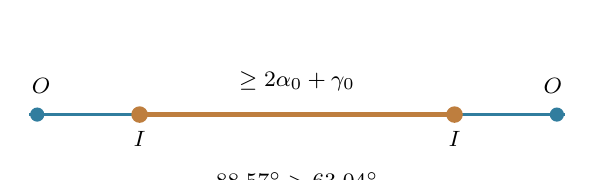
\begin{tikzpicture}[scale=1]
\draw[sea,very thick] (-3.4,0)--(3.4,0);
\node[figlabel] at (-3.25,.37) {$O$};\node[figlabel] at (3.25,.37) {$O$};
\draw[amber,line width=1.5pt] (-2.0,0)--(.25,0)--(2.0,0);
\fill[sea] (-3.3,0) circle (.09);\fill[sea] (3.3,0) circle (.09);
\fill[amber] (-2,0) circle (.105);\fill[amber] (2,0) circle (.105);
\node[figlabel] at (-2,-.31) {$I$};\node[figlabel] at (2,-.31) {$I$};
\node[figlabel] at (0,.42) {$\ge 2\alpha_0+\gamma_0$};
\node[figlabel] at (0,-.85) {$88.57^\circ>63.04^\circ$};
\end{tikzpicture}
\caption{外側ギャップに内側円が2個ある場合の角度矛盾。図中の距離は角度下界の和を表す模式図。}
\end{figure}

\begin{lemma}[中心半径 $\azero$ 以下の5円は正五角形]\label{lem:pentagon}
5つの単位円が、中心半径 $\le\azero$ にあり、互いに重ならないなら、
5中心は原点を中心とする半径 $\azero$ の正五角形の頂点にある。
\end{lemma}
\begin{proof}
5つの中心を偏角順に並べる。少なくとも1つの隣接偏角差は $2\pi/5$ 以下である。
任意の $0\le x,y\le\azero$ と $0\le\Delta\le2\pi/5$ について
\[
 D^2=x^2+y^2-2xy\cos\Delta
 \le \max\{\azero^2,\,2\azero^2(1-\cos(2\pi/5))\}=4.
\]
これは、$D^2$ が正方形 $[0,\azero]^2$ 上の凸関数なので、その最大値を
四隅で比較したものである。$\azero^2<4$ であり、等号 $D=2$ は
$x=y=\azero,\Delta=2\pi/5$ のときにしか起きない。
従って、非重複のためすべての隣接偏角差が $\ge2\pi/5$ でなくてはならず、
総和 $2\pi$ から5つとも $2\pi/5$ に等しい。
すべての中心半径も $\azero$ となる。
\end{proof}
\begin{theorem}[すべての内側半径が $\azero$ 以下なら排除]\label{thm:low}
内側5円・外側10円の配置が $R\le\Rc$ で実現可能であり、
\[
 a_i\le\azero\qquad(i=1,\ldots,5)
\]
ならば $R=\Rc$ である。特に $R<\Rc$ は不可能である。
\end{theorem}
\begin{proof}
\Cref{lem:pentagon}により内側5円は半径 $\azero$ の正五角形をなす。
隣接する内側2中心の偏角差は $2\pi/5=72^\circ$ である。
外側10円を中心半径 $\bzero$ に移して考えると、
この72度の区間に外側円が3個以上入る場合、必要角度は
$2\alpha_0+2\thzero>72^\circ$ となり不可能である。
5区間に外側10円を分けるため、各区間には\emph{ちょうど2個}必要である。
各区間の必要角度は $2\alpha_0+\thzero=72^\circ$ に等しいため、
すべての内外・外外の接触角条件が等号となる。
したがって壁面化後の外側10円は、対応する内側円との距離がちょうど2である。
$R<\Rc$ なら元の外側円の中心半径は $\bzero$ 未満なので、
壁面化前の距離は厳密に2未満となり、非重複に反する。
\end{proof}
\begin{corollary}[残存する5+10型は半径が両側へ跨がる]\label{cor:mixed}
$R<\Rc$ の実現可能配置が内側5円・外側10円に属するなら、
\[
\boxed{\min_i a_i<\azero<\max_i a_i}
\]
が必要である。
\end{corollary}
\begin{figure}[H]\centering
\begin{tikzpicture}[x=.86cm,y=.84cm]
\draw[ink,-{Latex}] (0,0)--(10.1,0) node[right,figlabel] {内側半径 $a_i$};
\fill[amber!14] (0,.45) rectangle (3.2,1.38);
\fill[red!7] (3.2,.45) rectangle (6.15,1.38);
\fill[sea!14] (6.15,.45) rectangle (9.4,1.38);
\draw[ink!60,densely dashed] (3.2,.2)--(3.2,1.7);
\draw[ink!60,densely dashed] (6.15,.2)--(6.15,1.7);
\node[font=\small] at (1.55,.92) {全 $a_i\le a_0$};
\node[font=\small] at (4.69,.92) {混合領域};
\node[font=\small] at (7.82,.92) {全 $a_i\ge a_0$};
\node[font=\small,text=alert] at (1.55,1.88) {排除済};
\node[font=\small,text=alert] at (7.82,1.88) {排除済};
\node[font=\small,text=ink] at (4.69,1.88) {未解決};
\end{tikzpicture}
\caption{5+10型の残存条件の模式図。中央の混合領域には近傍障壁で排除できる部分もある。}
\end{figure}

\section{混合領域の局所障壁と負閉路}
内側5円が各々異なる外側ギャップに入り、巡回順序が $(I,O,O)^5$ の場合、
半径 $a_i$ に対して
\[
 h_i=\Phi(a_i,a_{i+1}),\qquad
 k_i=\Phi(a_i,\bzero)+\thzero+\Phi(a_{i+1},\bzero)
\]
を定義する。必要角度制約は、近傍では
\begin{equation}\label{eq:localbarrier}
 \sum_{i=1}^5\max\{h_i,k_i\}\le2\pi
\end{equation}
である。$a_i=\azero$ では $h_i=k_i=2\pi/5$。
\begin{proposition}[奇数サイクルによる局所障壁]\label{prop:local}
ある $\eta>0$ が存在して、$|a_i-\azero|<\eta$ をすべての $i$ が満たす
$(I,O,O)^5$ 型の配置に対して $R<\Rc$ は不可能である。
\end{proposition}
\begin{proof}[証明の概略]
$\delta_i=a_i-\azero$, $\sigma_i=\delta_i+\delta_{i+1}$ とおく。
$\delta_i=0$ の近傍で
\begin{align*}
 h_i&=\frac{2\pi}{5}-c\sigma_i+O(\|\delta\|_1^2),\\
 k_i&=\frac{2\pi}{5}+d\sigma_i+O(\|\delta\|_1^2),
\end{align*}
ただし $c=\sin^2(\pi/5)/\cos(\pi/5)>0$、$d=\cos(\pi/5)>c$ である。
\[
\sum_i\max(h_i,k_i)\ge2\pi+c\sum_i|\sigma_i|-C\|\delta\|_1^2.
\]
5という奇数個の巡回構造から
$2\delta_i=\sigma_i-\sigma_{i+1}+\sigma_{i+2}-\sigma_{i+3}+\sigma_{i+4}$ なので、
$\sum_i|\sigma_i|\ge(2/5)\|\delta\|_1$ が成り立つ。
$\eta$ を十分小さくすると、$\delta\ne0$ で角度和は $2\pi$ を超える。
$\delta=0$ かつ $R<\Rc$ の場合は、外側円を壁面化して得た
接触角の等号と元の外側円の中心半径の厳密な小ささから排除される。
\end{proof}
\begin{figure}[H]\centering
\begin{tikzpicture}[scale=.95]
\foreach \k in {0,...,4}{\pgfmathsetmacro{\t}{90+72*\k}
\coordinate (V\k) at (\t:1.72);
\fill[amber] (V\k) circle (.11);
\node[font=\scriptsize,fill=white,inner sep=1pt] at (\t:2.13) {$\delta_{\k}$};}
\foreach \k in {0,...,4}{\pgfmathtruncatemacro{\n}{mod(\k+1,5)}
\draw[ink!70,thick] (V\k)--(V\n);
\path (V\k)--(V\n) node[pos=.52,fill=white,font=\scriptsize] {$\sigma_{\k}$};}
\node[font=\small,align=center] at (0,0) {$\sigma_i=\delta_i+\delta_{i+1}$\\奇数サイクル};
\node[font=\small,align=left,anchor=west] at (2.65,.6) {$\sigma_i=0$ が全辺で成立\\ $\Longrightarrow\delta_i=0$};
\end{tikzpicture}
\caption{局所障壁の核心。5サイクル上で隣接摂動の和が消えるのは、自明な摂動のみ。}
\end{figure}
\Cref{prop:local}は接触構造を仮定した\emph{局所}定理である。
一般の半径ベクトルでは、角度差制約
\[
 \gamma_{ij}\le\theta_j-\theta_i\le2\pi-\gamma_{ij}
\]
を全円対で組み、負閉路で排除する方法が必要になる。
\begin{figure}[H]\centering
\begin{tikzpicture}[>=Latex,node distance=2cm]
\node[flowbox] (a) at (0,0) {$\theta_i$};
\node[flowbox] (b) at (3,0) {$\theta_j$};
\draw[sea,thick,->,bend left=27] (a) to node[above,font=\footnotesize] {$2\pi-\gamma_{ij}$} (b);
\draw[amber,thick,->,bend left=27] (b) to node[below,font=\footnotesize] {$-\gamma_{ij}$} (a);
\node[font=\small,align=left,anchor=west] at (5.2,0) {閉路重みが負\\$\Longrightarrow$ 実現不可能};
\end{tikzpicture}
\caption{角度差制約の2本の有向辺。全ペアの辺と巡回順序制約を合わせ、負閉路を探索する。}
\end{figure}

\section{全配置を閉じるために残る計算}
内側が $k=5,6,7,8$ 個の場合、内外二値巡回語の二面体群同値類は以下の760個となる
（第1ノートで説明したBurnsideの補題による）。
\begin{table}[H]\centering
\caption{残る構造分類と自由中心半径の数。}
\begin{tabular}{@{}cccc@{}}\toprule
内側 $k$ & 外側 $15-k$ & 巡回パターン数 & 自由中心半径\\\midrule
5 &10&111&5\\
6 &9&185&6\\
7 &8&232&7\\
8 &7&232&8\\\midrule
合計&--&760&最大8\\\bottomrule
\end{tabular}
\end{table}
\begin{problem}[大域被覆の最終課題]\label{problem:global}
\eqref{eq:feasibility}で $R<\Rc$ を満たす実現可能配置が存在しないことを、
760個すべての巡回クラスおよび各 $k$ 次元の半径区間について厳密に示せ。
特に、次の残存領域を扱う必要がある：
\begin{itemize}
\item $k=5$、$\min a_i<\azero<\max a_i$ の\emph{非局所}混合領域；
\item $k=5$ でも巡回順序が $(I,O,O)^5$ でないクラス；
\item $k=6,7,8$ の全巡回クラス。
\end{itemize}
\end{problem}
\begin{figure}[H]\centering
\begin{tikzpicture}[node distance=1.3cm,>=Latex]
\node[flowbox,text width=10cm] (all) at (0,0) {15円の任意配置、$R\le R_0$};
\node[flowbox,text width=10cm] (wall) at (0,-1.0) {外側円を $b_0$ まで一括壁面化（定理\ref{thm:radialpush}）};
\node[flowbox,text width=10cm] (types) at (0,-2.0) {内側 $k=5,6,7,8$ ／ 二面体同値類760個};
\node[flowbox,text width=10cm] (bounds) at (0,-3.0) {各クラスで順位上下界を適用し、$k$ 変数の半径箱へ};
\node[flowbox,text width=10cm] (try) at (0,-4.0) {角度負閉路・距離矛盾・局所障壁・半径箱の再分割};
\node[draw=alert,fill=red!3,rounded corners=2pt,minimum width=10.3cm,align=center,font=\sffamily\small] (open) at (0,-5.0) {現時点：すべての箱を閉じる有限証明書は未作成};
\foreach \u/\v in {all/wall,wall/types,types/bounds,bounds/try,try/open}{\draw[ink!75,thick,->] (\u)--(\v);}
\end{tikzpicture}
\caption{厳密な推論規則と、依然として未実行の大域被覆計算を区別した証明フロー。}
\end{figure}
\subsection{検証器に追加すべき推論規則}
\begin{enumerate}
\item \texttt{WALL\_PUSH}: 半径 $\ge L$ の中心を壁面へ固定する変形の健全性を確認する。
\item \texttt{ORDER\_BOUND}: $s_{(k)}$ に関する下界\eqref{eq:orderlower}・上界\eqref{eq:um}を適用する。
\item \texttt{GAP\_BUDGET}: 外側10円のギャップ和と、内側円の挿入費用を比較する。
\item \texttt{SAME\_SIDE}: 5+10型で全 $a_i\ge\azero$ または全 $a_i\le\azero$ を排除する。
\item \texttt{NEGATIVE\_CYCLE}: 有理区間上で閉路重みの厳密な負値を検証する。
\item \texttt{SPLIT}: 各半径箱を端点共有の2つの閉区間へ分割する。
\end{enumerate}
実装には $R_0$ と三角関数値の厳密な代数的定義、外向き丸めまたは有理区間評価、
全分岐の被覆検証が必要である。浮動小数点で負閉路が見つかった事実のみでは証明にならない。

\section{結論：何が進み、何が残ったか}
\begin{statusbox}
\textcolor{mint}{\textbf{本ノートで証明したこと}}\par
(1) 外側円の一括壁面化；
(2) 中心半径順位の明示的上界；
(3) 内側5円・外側10円の「全て $\azero$ 以上」「全て $\azero$ 以下」の大域排除；
(4) 5+10型の非対称摂動に対する局所角度障壁の再整理。\par
\textcolor{alert}{\textbf{残ったこと}}\par
混合領域と内側6--8円の全ケースについて、有限の厳密排除証明書を生成・検証すること。
\end{statusbox}
したがって、本ノートは15等円の最適性を証明する論文ではない。
一方、半径15変数から最大8変数への削減、外周角度予算の逼迫、
5+10型に対する大域的排除領域の拡大は、今後の計算機援用証明の有用な基盤となる。

\begin{thebibliography}{9}
\bibitem{packomania} E.~Specht, \emph{The best known packings of equal circles in a circle},
Packomania, \url{https://www.packomania.com/cci/cci.html} (閲覧：2026-10-09).
\bibitem{ekanayake} D.~B. Ekanayake and D.~J. LaFountain,
\emph{Tight partitions for packing circles in a circle},
Italian Journal of Pure and Applied Mathematics \textbf{51} (2024), 115--136.
\url{https://ijpam.uniud.it/online_issue/202451/10%20Ekanayake-LaFountain.pdf}.
\end{thebibliography}
\end{document}
